\chapter{Struktura aplikacji MobiNote}

Struktura aplikacji MobiNote została częściowo opisana w \ref{ch:manual} rozdziale.

\section{Notatki}

Każda notatka składa się z nagłówka (tytułu) oraz zawartości.
Nagłówkiem jest tekst edytowany w polu tekstowym znajdującym się w górnym pasku strony, natomiast zawartość notatki jest ciągiem akapitów dodawanych, edytowanych i usuwanych w edytorze notatki. Akapity mogą przechowywać tekst, jak również widgety. Struktura kodu opiera się na wzorcu MVC (Model View Controller), którą można przedstawić w uproszczony sposób za pomocą schematu:

\begin{figure}[ht]
    \centering
    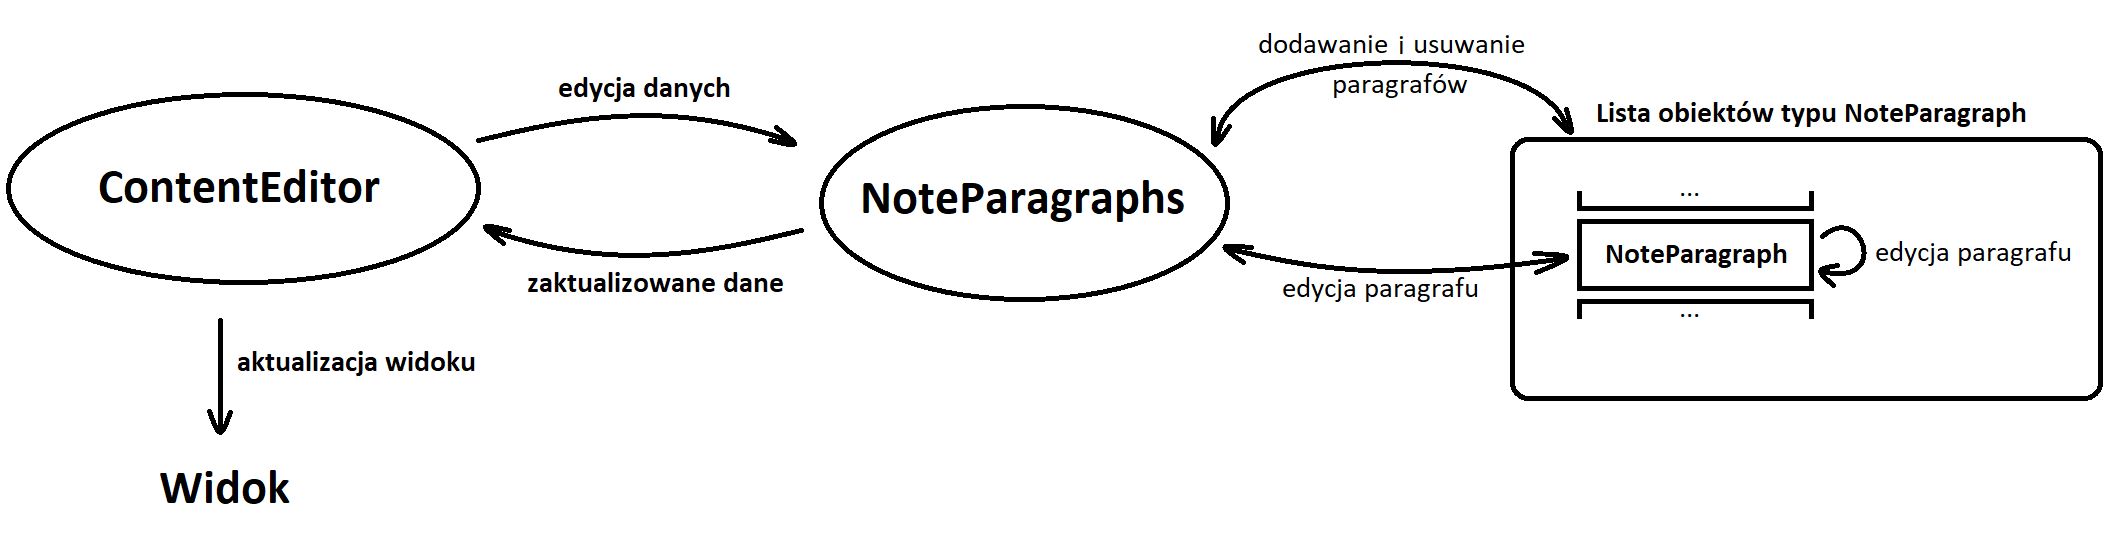
\includegraphics[width=\linewidth]{images/ContentEditor_podzial.png}
    \caption{Uproszczony schemat struktury i działania edytora notatki.}
\end{figure}

W obecnej implementacji aplikacji \textbf{MobiNote} za widok odpowiada obiekt klasy \textbf{ContentEditor}, natomiast kontrolerem danych jest obiekt klasy \textbf{NoteParagraphs}, który również przechowuje dane składające się na model. Jest to świadomy zabieg. Model nie jest skomplikowany i rozbudowany, dlatego też nie trzeba tworzyć dodatkowych struktur i klas do zarządzania nim, jak w klasycznym wzorcu MVC. Pozwala to na uproszczenie logiki i struktury kodu, mniejsze wykorzystanie pamięci, oraz skrócenie ścieżki wywołań w przypadku wykonywania konkretnych operacji na danych. Zabieg ten został użyty z myślą o użytkownikach korzystających z mniej wydajnych urządzeń.

\section{Przechowywanie notatki}

Zawartość notatki przechowywana jest jako lista akapitów w obiekcie klasy \textbf{NoteParagraphs}. Każdy akapit jest obiektem klasy dziedziczącej po klasie \textbf{NoteParagraph}. W przypadku akapitów tekstowych zawartością przechowywaną w obiekcie będzie tekst, natomiast w przypadku akapitów widgetów będą to parametry widgetów zawartych w danym akapicie. Ten model danych jest zapisywany w bazie danych w odpowiednim formacie oraz odczytywany i konwertowany z powrotem wraz z przejściem do strony edycji danej notatki.

\subsection{Akapity}

Istnieją trzy typy akapitów w edytorze dziedziczące po \textbf{NoteParagraph}: 
\begin{itemize}
    \item \textbf{NoteParagraphTextEditor};
    \item \textbf{NoteParagraphWidget};
    \item \textbf{NoteParagraphPlaceholder}.
\end{itemize}

Schemat dziedziczenia wygląda następująco:

%------- UML---------
% niestety kompilator daje bledy, gdy chce uzyc:
% \usepackage{tikz}
% \usepackage{pgfplots}
% \usepackage[simplified]{pgf-umlcd}
% dlatego uzyje zdjecia skompilowanego diagramu w innym projekcie

% \renewcommand{\umltextcolor}{black}
% \renewcommand{\umlfillcolor}{white}
% \renewcommand{\umldrawcolor}{black}

% \begin{tikzpicture}[scale=0.7, every node/.style={transform shape},
% rounded corners=2pt]

% \begin{abstractclass}{NoteParagraph}{5.5,3}
% \attribute{+ noteWidgetFactory : \mbox{NoteEditorWidgetFactory}}
% \attribute{+ id : int}

% \operation[0]{+ onContentChange()}
% \operation[0]{+ reportFocusParagraph()}
% \operation[0]{+ deleteParagraph()}
% \operation[0]{+ requestFocus()}
% \operation[0]{+ setDefaultCallbacks()}

% \operation[0]{+ get content : String}
% \operation[0]{+ get rawLength : int}
% \operation[0]{+ get widgetTree : String}
% \operation[0]{+ get str : String}
% \end{abstractclass}

% \begin{class}{NoteParagraphTextEditor}{0,-6}
% \inherit{NoteParagraph}
% \attribute{+ cursor : int}
% \attribute{+ fontSize : int}
% \attribute{+ paragraphText : String}

% \operation[0]{+ addParagraph()}
% \operation[0]{+ addPlaceholder()}
% \operation[0]{+ append()}
% \end{class}


% \begin{class}{NoteParagraphWidget}{5.5,-6}
% \inherit{NoteParagraph}
% \attribute{+ widgetJSON : String}
% \attribute{+ mode : WidgetMode}
% \attribute{+ elements : \mbox{List$<$NoteEditorWidget$>$}}

% \operation[0]{+ \mbox{addWidget()}}
% \operation[0]{+ \mbox{addWidgetByData()}}
% \operation[0]{+ setMode()}
% \operation[0]{+ removeFromParent()}
% \end{class}


% \begin{class}{NoteParagraphPlaceholder}{11,-6}
% \inherit{NoteParagraph}
% \operation{+ onTap()}
% \end{class}

% \end{tikzpicture}

%--------UML---------

\begin{figure}[ht]
    \centering
    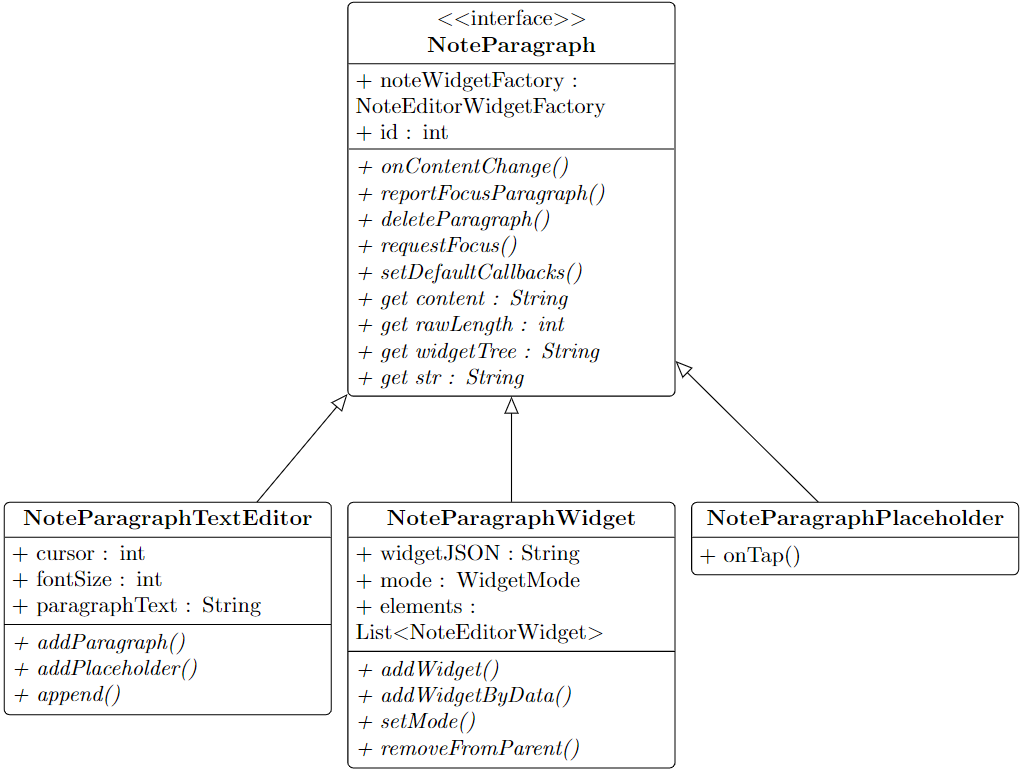
\includegraphics[width=\linewidth]{images/UML_klas.png}
    \label{fig:uml}
\end{figure}

\newpage

Każdy z akapitów posiada unikatowy identyfikator \texttt{id} oraz referencję do fabryki widgetów tworzonej wewnątrz managera \textbf{NoteParagraphs}.
Pozwala to na unikatowe identyfikowanie akapitów wewnątrz listy, oraz wszystkich utworzonych widgetów w obrębie przestrzeni edytora.

Używane są również mechanizmy wywołań zwrotnych (callbacks) do zgłaszania aktywności (focus), zaistniałej zmiany, jak również usunięcia samego siebie z listy akapitów, na podstawie własnego \texttt{id}, gdy wszystkie jego elementy zostaną usunięte.

\subsubsection{NoteParagraphTextEditor}

Służy do przechowywania, wyświetlania i edycji tekstu notatki. Posiada mechanizmy dynamicznej zmiany rozmiaru poprzez manipulację stanem oraz wartościami wewnętrznych pól. Posiada tylko jeden element, którym jest pole tekstowe z niestandardowym kontrolerem \textit{NoteTextEditingController} parsującym tekst przy użyciu własnego parsera.

\subsubsection{NoteParagraphWidget}

Służy do przechowywania, wyświetlania i edycji widgetów notatki. Posiada mechanizmy dynamicznej zmiany rozmiaru wraz ze zmianą rozmiaru widgetu będącego elementem głównym. Mechanizmy zmiany rozmiaru są różne w zależności od rodzaju widgetu.

\subsubsection{NoteParagraphPlaceholder}

Służy jako wypełnienie pozostałej przestrzeni edytora. Po kliknięciu na niego uruchamia mechanizm przenoszenia aktywności (focus) na ostatni akapit na liście, dzięki czemu użytkownik nie musi znać wielkości i szukać ostatniego akapitu, aby kontynuować edycję notatki.

\newpage

\subsection{Widgety}

W aktualnej wersji aplikacji widgety dzielą się na:
\begin{compactitem}
    \item widgety główne (będące bezpośrednimi elementami \textbf{NoteParagraphWidget})
    \item widgety będące elementami widgetów głównych.
\end{compactitem}
W przypadku rozwoju aplikacji struktury widgetów oraz ich hierarchii i tworzenia ulegną zmianie. Aktualnie struktura aplikacji wygląda następująco:

\begin{figure}[ht]
    \centering
    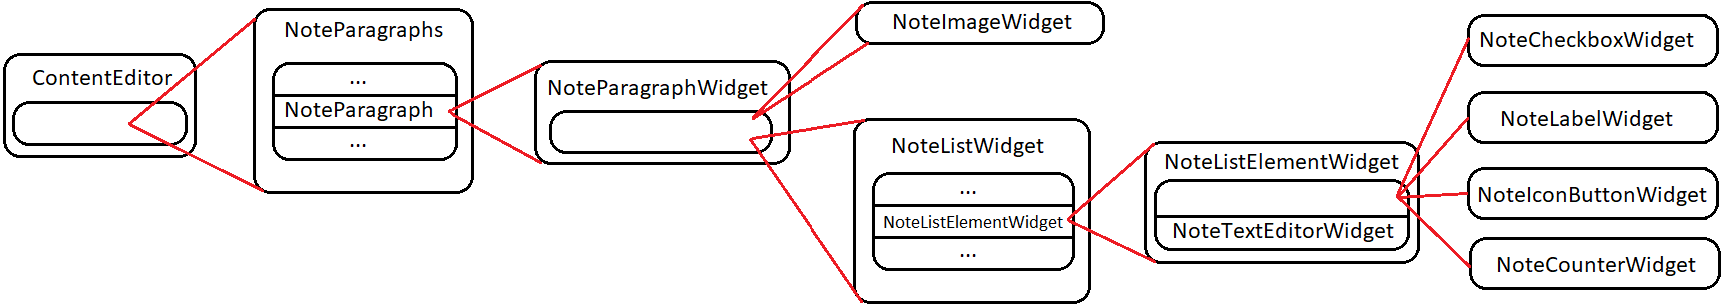
\includegraphics[width=\linewidth]{images/struktura_widgetow_w_notatce.png}
    \caption{Struktura widgetów zawartości notatki w aktualnej wersji aplikacji.}
    \label{fig:struktura-widgetow}
\end{figure}

Widgety przechowywane są w modelu za pomocą obiektów klas pochodznych od klasy \textbf{NoteWidgetData}. Każdy używany typ widgetu posiada opisujący go typ danych \textbf{NoteWidgetData}. Wszystkie dostępne typy danych dostępne są w plikach w katalogu \textit{lib/logic/note\_{}editor/widgets/representation/}. Dane te zostają zapisane w bazie danych w formacie JSON.

\section{Parsowanie notatki}

\subsection{Problem parsowania tekstu ze znacznikami stylu}

Do wyświetlania stylizowanego tekstu potrzebne jest jego parsowanie. Funkcjonalność ta będzie wołana stosunkowo często, a dla długich tekstów bez znaku nowej linii będzie to długi do obsługi tekst. Dlatego też ważny jest sposób implementacji.

Zrealizowanym pomysłem rozwiązania problemu jest podział parsowania tekstu na trzy etapy:
\begin{enumerate}
    \setlength\itemsep{0mm}
    \item przekształcanie znaczników stylu w tekście na \textbf{znaki unicode};
    \item parsowanie tekstu ze \textbf{znakami unicode} na specjalną drzewiastą reprezentację \textbf{SpanInfo};
    \item konwersja struktury \textbf{SpanInfo} na obiekt \textbf{TextSpan}.
\end{enumerate}

\subsection{Implementacja parsera}

\subsubsection{Własna implementacja}

Parser wraz z jego strukturą został zaprojektowany i zaimplementowany przeze mnie, zamiast przy użyciu narzędzi generowania parsera dla opisanej gramatyki używanego przeze mnie języka znaczników. Powodem tego jest potrzeba łatwego rozwoju oraz wprowadzenia niestandardowych rozwiązań i dodatkowych funkcjonalności niebędących częścią samej składni gramatyki, jednak potrzebnych wewnątrz implementacji parsera.

Własna implementacja parsera pozwoliła mi od początku do końca zaprojektować i zrozumieć jego strukturę, co pozwoliło mi tworzyć elastyczne środowisko rozwoju tekstu w notatkach. Przykładowo wprowadzanie funkcji odkrywania i ukrywania znaczników stylu oraz nagłówka, bądź dodanie wywołania zwrotnego zmieniającego rozmiar pola tekstowego było prostym zabiegiem niewymagającym dużych zmian i rozszerzeń kodu parsera.

\subsubsection{Parsowanie}

Każdy z etapów parsowania jest realizowany poprzez obiekt innej klasy. Całość łączona jest w metodzie obiektu \textbf{NoteTextEditingController}.
\newline
\begin{figure}[ht]
    \centering
    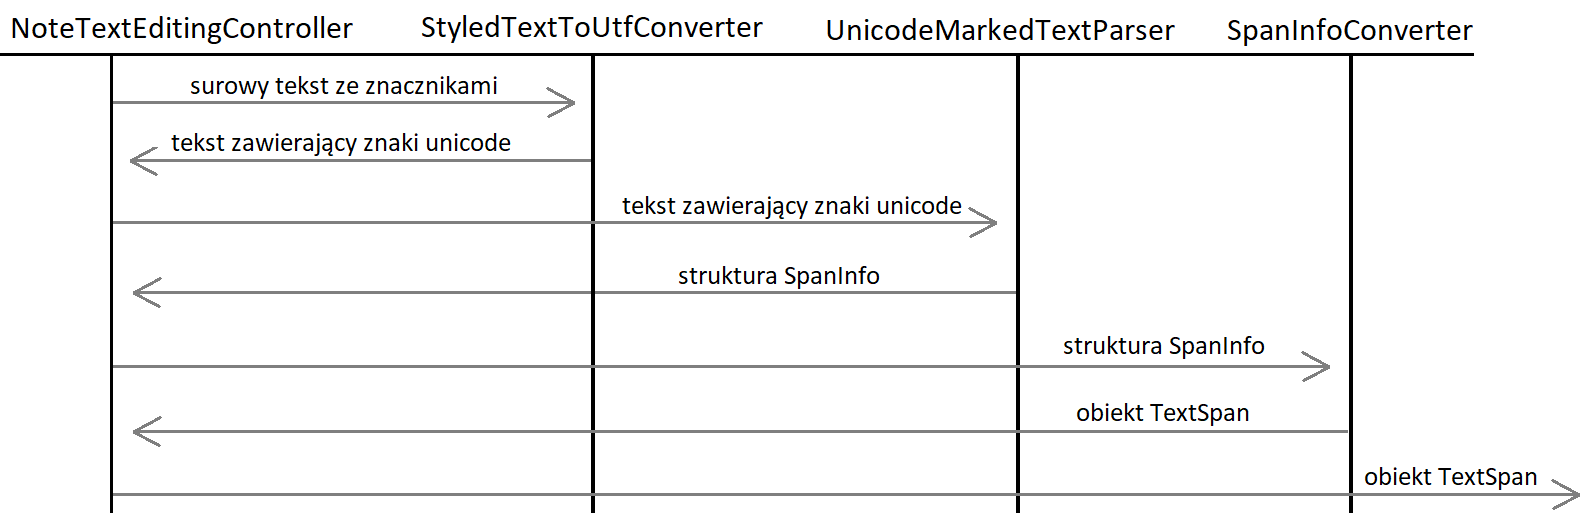
\includegraphics[width=\linewidth]{images/etapy_parsowania.png}
    \caption{Schemat przedstawiający etapy parsowania tekstu.}
    \label{fig:etapyParsowania}
\end{figure}

\subsubsection{Znaki unicode}

%https://unicode.org/glossary/#private_use_area
Do procesu parsowania zostały użyte znaki unicode z bloku Private Use Area. Są to znaki, które są trudno dostępne dla użytkownika z poziomu klawiatury mobilnej.

\noindent Zdefiniowane zostały w następujący sposób:

\begin{lstlisting}[language=java]
const styleUnicodeNumber = 0xe000;
const widgetUnicodeNumber = 0xe100;
const elementUnicodeNumber = 0xe1A0;
const paragraphUnicodeNumber = 0xe200;
\end{lstlisting}

Oznaczają odpowiednio początki przestrzeni znaczników: stylu tekstu, wewnętrznych widgetów i elementów w tekście oraz nagłówków akapitu.
Znaczniki początkowe mają parzyste numery, natomiast znaczniki końcowe mają nieparzyste numery następujące po odpowiadających im znacznikach początkowych.


\subsubsection{Struktura SpanInfo}

Podczas implementacji użyta została struktura \textbf{SpanInfo}. Zawiera ona informacje na temat danego węzła w drzewiastej strukturze stylów tekstu, oraz referencję do jego rodzica.
Została zaimplementowana w celu usprawnienia przebiegu etapu drugiego parsowania tekstu.

\begin{lstlisting}[language=java]
class SpanInfo {
  String type;
  String text;
  List<SpanInfo> children;
  late SpanInfo parent;
}
\end{lstlisting}

Dzięki swojej budowie struktura może zostać przekonwertowana w prosty sposób na obiekt typu \textbf{TextSpan}.

\subsubsection{StyledTextToUtfConverter}

Przekształcanie znaczników odbywa się poprzez przejście przez surowy tekst w ich poszukiwaniu i przetwarzaniu. Znaczniki dzielone są na początkowe i końcowe (zobacz: \ref{subsec:ustawianieStyli}). Podczas sprawdzania, czy dany znak jest znacznikiem początkowym, czy końcowym pobierany jest szerszy kontekst, złożony z przylegających do niego znaków.

W momencie, gdy zostanie znaleziony znak będący początkowym znacznikiem, dodawana jest informacja o nim do listy \textbf{startBounds} w postaci struktury \textbf{SpecialPatternInfo} przechowującej znacznik wraz z jego indeksem.

\begin{lstlisting}[language=Java]
class SpecialPatternInfo {
  final int indexInText;
  final String character;
}
\end{lstlisting}

W przypadku znalezienia znaku $c$ będącego końcowym znacznikiem, przeszukujemy listę \textbf{startBounds} w poszukiwaniu pierwszego wystąpienia znacznika $c'$ o takiej samej wartości. Jeśli nie zostanie znaleziony, wówczas znak $c$ traktowany jest jako zwykły tekst. Jeśli natomiast zostanie znaleziony, oznacza to, że wystąpił wcześniej początek stylu, a cały tekst pomiędzy aktualnym indeksem, a indeksem zapisanym w strukturze opisującej początkowy znacznik $c'$ jest tekstem zawierającym ten styl. Zatem znalezione znaczniki zamieniane są na swoje odpowiedniki w formie znaków unicode, a znaczniki istniejące na liście \textbf{startBounds} będące następnikami znalezionego $c'$ zostają usunięte z listy (granice stylów nie mogą się przecinać), a więc nie zostaną zamienione.

W podobny sposób konwertowane są również widgety i elementy wewnętrzne w tekście. W aktualnej wersji aplikacji nie są one obsługiwane, jednak sam parser został przygotowany na obsługę tego typu problemu. Szukane są zatem również fragmenty tekstu będące tagami widgetów, bądź oznaczeniami elementów.

\subsubsection{UnicodeMarkedTextParser}

Z racji tego, ze znaki unicode z zakresu Private Use Area są trudno dostępne, na potrzeby samego problemu konwersji tekstu notatek możemy założyć, że znaki w tekście symbolizują początkowe i końcowe znaczniki, które na pewno mają swoje odpowiedniki i są poprawnie użyte (nie przecinają się).

Na początku algorytmu tworzona jest referencja $currentSpan$ na obiekt \textbf{SpanInfo}, który jest aktualnie przetwarzanym stylem (napotkany został jego znacznik początkowy). Początkowo jest to korzeń całej struktury \textbf{SpanInfo}.

Oznaczony w ten sposób tekst przechodzimy ponownie posiadając dokładne informacje, które symbole są znacznikami stylu, a które zwykłymi fragmentami tekstu.

Podczas przechodzenia tekstu zapisujemy znaki niebędące znacznikami do tymczasowego bufora.

Napotykając znacznik początkowy, jeśli w buforze znajduje się tekst, to wówczas jest on dodawany do tekstu przechowywanego w $currentSpan$. Następnie tworzony jest nowy \textbf{SpanInfo} (na podstawie stylu reprezentowanego przez znacznik) będący dzieckiem $currentSpan$. Następnie referencja do nowo powstałego obiektu zapisywana jest jako $currentSpan$. 

Po napotkaniu znacznika końcowego dodajemy tekst z tymczasowego bufora do $currentSpan$, czyścimy bufor i przestawiamy $currentSpan$ przechodząc po węzłach \textbf{SpanInfo} (używane jest do tego pole z referencją $parent$ wskazującą na rodzica danego węzła) na pierwszy napotkany węzeł przechowujący informacje na temat stylu reprezentowanego przez aktualnie sprawdzany znacznik.

Przetwarzane są również informacje na temat widgetów i elementów wewnętrznych przygotowane w ramach podstawy do rozwoju funkcjonalności w przyszłości.

\subsubsection{SpanInfoConverter}

Klasa \textbf{TextSpan} jest klasą pochodną klasy \textbf{InlineSpan}.

\textbf{SpanInfoConverter} buduje strukturę \textbf{InlineSpan} złożoną z obiektów klas pochodnych \textbf{TextSpan} oraz \textbf{WidgetSpan}. Wewnętrzne widgety i elementy, które mają w przyszłości być obsługiwane przy użyciu \textbf{WidgetSpan} nie są aktualnie obsługiwane, dlatego przyjęty w opisie model struktury opiera się tylko na obiektach typu \textbf{TextSpan}.

Przechodząc przez strukturę \textbf{SpanInfo} budujemy strukturę złożoną z obiektów typu \textbf{TextSpan}. Zapisywany jest $mainSpan$ będący korzeniem struktury, natomiast przejście przez strukturę odbywa się w sposób rekurencyjny.

\begin{lstlisting}[language=Java]
SpanInfo mainSpan = SpanInfo(type: 'null');

InlineSpan getSpans(SpanInfo spanInfo) {
    if (mainSpan.type == 'null') mainSpan = spanInfo;

    List<InlineSpan> spanChildren =
        spanInfo.children.map((e) => getSpans(e)).toList();

    /* ustawianie stylu i typu obiektu 
     * oraz zwracanie go wraz z children */
}
\end{lstlisting}

\newpage

\section{Prezentowanie notatki}

Za widok notatki odpowiada klasa \textbf{ContentEditor}. Pozwala ona na wyświetlanie zawartości akapitów oraz ich elementów, jak również za jej pośrednictwem użytkownik może edytować notatkę z poziomu widoku.

\subsection{Widgety}

\subsubsection{Tworzenie widgetów}

Widgety tworzone są poprzez interakcję użytkownika przy użyciu interfejsu użytkownika (patrz \ref{sub:dodawanieWidgetow}), jak również poprzez przetwarzanie zawartości notatki z bazy danych. W obu przypadkach tworzone są odpowiednie obiekty typu \textbf{NoteWidgetData} na podstawie użytej funkcjonalności bądź przetworzonych danych pobranych z bazy danych. Na ich podstawie tworzone są widgety wyświetlane w edytorze.

\begin{figure}[ht]
    \centering
    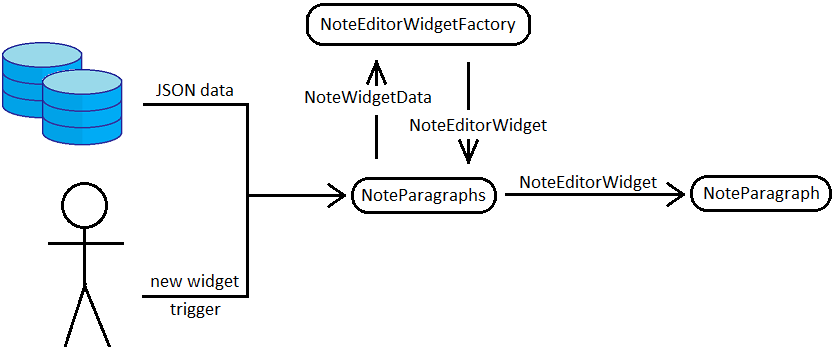
\includegraphics[height=5cm]{images/tworzenie_widgetow.png}
    \caption{Schemat tworzenia widgetów.}
    \label{fig:create-widget}
\end{figure}

\subsubsection{Usuwanie widgetów}

Widgety usuwane są poprzez interakcję użytkownika z dostępnym interfejsem graficznym po przejściu w tryb zaznaczenia (patrz \ref{sub:usuwanieWidgetow}). Widgety usuwane są w swoich rodzicach, a jeśli brakuje widgetów potomnych, wówczas widget listy bądź akapit widgetów zostaje usunięty.

\newpage

\subsection{Tekst}

Praca z tekstem dzieli się na edycję tekstu z użyciem logiki zawartej w \textbf{NoteParagraphTextEditor} i \textbf{NoteTextEditorWidget}, jak również wyświetlanie go wraz ze zmianą rozmiarów z pomocą \textbf{NoteTextEditingController}.

Tekst edytowany jest za pomocą pola tekstowego TextField udostępnianego jako widget przez framework flutter. Posiada on wewnętrzny padding poziomy (lewa i prawa strona) jako stałą wartość, oraz padding pionowy (góra, dół) obliczany na podstawie różnicy pomiędzy wielkością czcionki użytej w danym akapicie, a domyślnej czcionki z dodatkiem podstawowej wartości niezerowej (w przypadku, gdy dany akapit nie ma ustawionego nagłówka, nie chcemy braku odstępu między akapitami z powodu zerowego paddingu pionowego).

Przy każdej zmianie tekstu sprawdzana jest jego zawartość w poszukiwaniu informacji o stanie akapitu. Stan ten określa się poprzez wielkość czcionki i stylów tekstu użytych w akapicie.

\subsubsection{Dodawanie tekstu}

Jeśli wewnątrz pola tekstowego został dodany znak nowej linii, wówczas wołane jest wywołanie zwrotne (callback), zainicjalizowane przy tworzeniu danego akapitu przez \textbf{NoteParagraphs}, służące do dodania nowego akapitu. Wywołanie to przyjmuje identyfikator danego akapitu i na tej podstawie oblicza miejsce w liście, do którego należy włożyć nowo powstały akapit. Przy tworzeniu nowego akapitu następuje przeniesienie tekstu następującego po znaku końca linii. Znak końca linii jest usuwany.

\subsubsection{Usuwanie tekstu}
\label{eq:usuwanieTekstu}

Flutter nie oferuje możliwości przechwycenia zdarzenia naciśnięcia przycisku \textbf{delete}, gdy kursor znajduje się na początku tekstu. W tej sytuacji najprościej jest użyć przechwycenia zdarzenia edycji tekstu w akapicie.

W każdym akapicie na początku dodawany jest znak \verb|placeholder = \u200b|. Jest to znak unicode reprezentujący spację o zerowej długości, a więc niewidoczną w tekście. Jest to swego rodzaju wartownik. Jego brak na początku tekstu podczas sprawdzania tekstu po edycji mówi o potrzebie usunięcia akapitu.

Gdy użytkownik zechce usunąć akapit, wówczas przenosi się kliknięciem na początek wiersza (o ile już się na nim nie znajduje), a następnie naciska przycisk \textbf{delete}. Dzięki temu usuwa \verb|placeholder|, a przy tym wywoływany jest callback służący do usunięcia akapitu. Jako argument przyjmuje identyfikator akapitu, aby określić miejsce usunięcia.

Aby uniknąć kliknięcia na początek linii przed wartownika został dodany mechanizm zmiany pozycji kursora na drugi znak (bezpośrednio za wartownikiem) za każdym razem, gdy jest on na pozycji zerowej.

\subsubsection{Wyświetlanie tekstu}

Do wyświetlania stylizowanego tekstu używane są obiekty typu \textbf{TextSpan}. Obiekty te posiadają drzewiastą strukturę, ponieważ mogą zawierać dzieci tego samego typu, które będą dziedziczyć dane parametry stylu, o ile nie zostaną dla nich specjalnie zainicjalizowane. Daje to możliwość zorganizowania tekstu bez potrzeby dzielenia go na małe kawałki oraz nadawania za każdym razem łączonych stylów (gdyby obiekty \textbf{TextSpan} były przechowywane jako elementy jednej listy). Można zainicjalizować jeden styl wewnątrz drugiego, co bardzo upraszcza strukturę i pozwala na wprowadzanie globalnych zmian struktury (jak na przykład wielkość czcionki całego akapitu) tylko w korzeniu, zapewniając, że wszystkie części tekstu odziedziczą zmianę.

Aktualizacja i renderowanie wyglądu pola tekstowego na bieżąco jest możliwe poprzez wykorzystanie klasy \textbf{TextEditingController}. Posiada ona metodę \textbf{buildTextSpan}, która służy do budowania wyglądu i stylu tekstu poprzez obiekty \textbf{TextSpan}. Dziedzicząc z tej klasy i nadpisując metodę \textbf{buildTextSpan} mogłem użyć parsera tekstu zawierającego znaczniki do przekonwertowania go na stylizowany tekst.
Dzięki temu przy każdej zmianie tekst jest parsowany, a jego wygląd aktualizowany.

Utworzony w ten sposób \textbf{NoteTextEditingController} może nie tylko używać parsera do tworzenia obiektów \textbf{TextSpan}, ale również mógł zostać rozszerzony o dodatkowe parametry, takie jak:

\begin{compactitem}
    \item callback \textbf{resizeTextField} wołany podczas parsowania, gdy wielkość czcionki w tekście ulega zmianie;
    \item możliwość przechowywania informacji o tym, czy dany akapit jest aktualnie w użyciu;
    \item sprawdzanie i manipulacja pozycją kursora.
\end{compactitem}

Callback \textbf{resizeTextField} został użyty w kontrolerze, zamiast w widgecie pola tekstowego, ponieważ wtedy wystarczy parsować tekst jednokrotnie. W momencie zwrócenia drzewiastej struktury tekstu \textbf{TextSpan} możemy ustawić rozmiar pola tekstowego w jego korzeniu, zamiast edytować zawartość widgetu używając innych mechanizmów i parsować dodatkowo tekst w poszukiwaniu informacji na temat wielkości czcionki.

Informacja na temat aktualnego użycia akapitu jest używana do wyświetlania i ukrywania znaczników stylu nagłówka.

Sprawdzanie i manipulacja pozycją kursora pozwala na odkrywanie znaczników stylu, jak również ustawianie pozycji, aby kursor nie znajdował się przed znakiem \verb|placeholder| (zobacz \ref{eq:usuwanieTekstu}).

Przy każdej zmianie tekstu odświeżany jest widok akapitu, dlatego wystarczy zmienić wartość zmiennej odpowiadającej za jego rozmiar przed końcem całej operacji związanej z przetwarzaniem nowego tekstu.
%https://api.flutter.dev/flutter/widgets/TextEditingController/buildTextSpan.html